 The game lasts for at most 23 rounds. In these 23 rounds, the flat hunters try to find the estate agent, while he tries to avoid them (this is because he would rather rent the flats to elderly couples, since presumably they make fewer parties in the middle of the night\ldots).\\

In each round, every player can make one move on the public transport system. The estate agent is the first, then it's the hunters' turn. One move is either 

\begin{itemize}
  \item  one or two stops by tram (colored lines),
  \item  one stop by train (thick orange lines),
  \item  or one stop by bus (thin light blue lines).
\end{itemize}

A move with a certain transport can only be made if one has still enough tickets (see \autoref{ticket_status}), if there is a connection (obviously), and if there is no other player at that destination (and in the case of tram lines, if there is no hunter in between).\\

 \textcolor{red}{Attention: If you are at a bus-only stop, and you run out of bus tickets, you will get stuck there forever, so be careful\ldots}\\

\begin{figure}[h]
  \centerline{\hbox{
    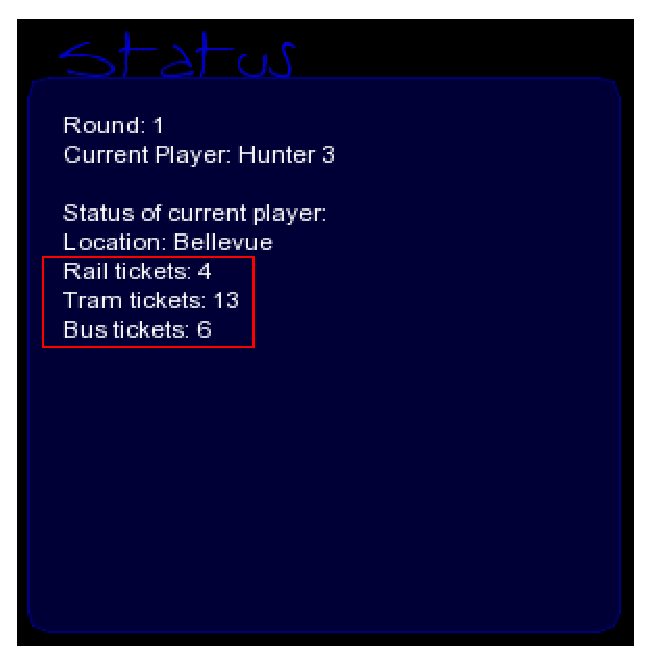
\includegraphics[width=50mm]{ticket_status}
  }}
\caption{Ticket status}
\label{ticket_status}
\end{figure}

The possible places you can move to are colored yellow (see \autoref{highlighted_places}). To make a move, just click on one of those highlighted places. The red circle centers on the player whose turn it is, and in the status box at the right, the game status and information about the current player get displayed. If you want to know the status of another player just click on his picture at the bottom. Click again to close the just opened status box.\\

\begin{figure}[h]
  \centerline{\hbox{
    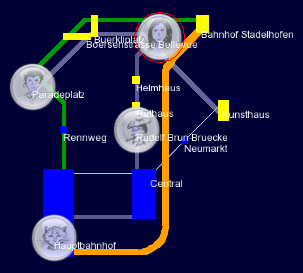
\includegraphics[width=50mm]{highlighted_places}
  }}
\caption{Highlighted places}
\label{highlighted_places}
\end{figure}

The game is over when

  \begin{description}
    \item[a)]the hunters could not find the estate agent within 23 rounds,
    \item[b)]one flat hunter moves onto the place where the agent currently is,
    \item[c)]or the hunters encircle the estate agent so that he cannot move anymore.
  \end{description}

In case a), the winner is the estate agent (he does not have to rent his flat to students), whereas in b) and c) it is the hunters that win, as they get to meet the estate agent on time and thus manage to find a flat.

